\documentclass[11pt]{article}
\usepackage[margin=1in]{geometry}
\usepackage{graphicx}
\usepackage{booktabs}
\usepackage{amsmath}
\usepackage{amssymb}
\usepackage{hyperref}
\usepackage{caption}
\usepackage{float}
\usepackage{xcolor}
\usepackage[ruled,linesnumbered]{algorithm2e}
\graphicspath{{../results/figures/}}
\hypersetup{colorlinks=true, linkcolor=blue, urlcolor=blue}

\title{\textbf{Accuracy Is Blind to Leakage, Interpretability Is Not:\\
Quantifying the Interpretability Leakage Gap on CWRU Bearing Diagnosis}}
\author{
Zekun Hu (202300620115) \and
Botao Gu (202300810014) \and
Zhiyang Gong (202300820063) \and
Guohao Fang (202300800150) \and
Changyang Wang (202300820133)
}
\date{July 2026}

\begin{document}
\maketitle

\begin{abstract}
Random-window splitting is a well-known data-leakage source for CWRU bearing fault
diagnosis, yet its severity is almost always judged through a single lens: classification
accuracy. We argue this lens is insufficient. On the full CWRU 12\,kHz drive-end dataset,
an envelope-spectrum 1D-CNN reaches $0.966\pm0.013$ accuracy under a random-window split
(protocol R) and $0.913\pm0.040$ under a leakage-safe recording-level split (protocol S),
a gap of only 5.3 points---small enough to be dismissed as seed noise. However, leakage
inflates the \emph{apparent} interpretability of the model far more visibly. Using
Grad-CAM over the envelope spectrum with a frequency-shift negative control, we define the
\textbf{Interpretability Leakage Gap} (ILG) as the difference in Grad-CAM margin
(true-band minus shifted-band saliency) between the two protocols. Over ten seeds we
measure $\mathrm{ILG}=+0.095$ (margin $0.263\pm0.015$ under R versus $0.168\pm0.028$ under
S), with a bootstrap $95\%$ confidence interval of $[0.079, 0.110]$ and a paired-$t$
$p=1.1\times10^{-6}$; the two protocols are completely separated on all ten seeds. We
trace the effect to memorization: test windows whose parent recording was seen during
training exhibit sharper apparent physical focus than windows from unseen recordings. The
effect transfers to a second, independent sensor location (the CWRU fan-end dataset), where
$\mathrm{ILG}=+0.048$ ($95\%$ CI $[0.022, 0.073]$, $p=0.008$). We conclude that mechanism
validation, not accuracy, is the reliable guard against leakage on saturated benchmarks.
All reported numbers are ten-seed means and are traceable to committed artifacts.
\end{abstract}

\section{Introduction}
Deep neural networks routinely report near-perfect accuracy on the Case Western Reserve
University (CWRU) bearing benchmark. Part of that success, however, is an artifact of how
the data are partitioned rather than a reflection of diagnostic ability. A CWRU recording
is a single long vibration time series; to obtain many training examples it is cut into
short, overlapping windows. If those windows are then shuffled and assigned to train and
test at random, near-identical neighbours from the same recording land on both sides of
the partition. A model can minimise its loss by recognising \emph{which recording} a
window came from rather than \emph{what fault} it contains (course manual, \S6.1).

The standard defence is a recording-level split, in which every window from a given
recording is confined to a single partition. The standard way to check whether leakage
mattered is to compare accuracy before and after adopting the safe split: a large drop is
taken as proof of leakage. We show that this diagnostic is unreliable on CWRU. Because the
four-class task is nearly saturated, both the leaky and the safe protocol score above
$0.91$, and the accuracy difference is comparable to the seed-to-seed variance. An analyst
who looked only at accuracy could reasonably, but wrongly, conclude that leakage is
harmless here.

Our central claim is that a second, more sensitive axis exists: the physical consistency
of the model's explanations. We ask whether leakage inflates not merely accuracy but the
\emph{appearance} of a physically grounded model. Concretely, does a model trained under a
leaky split produce Grad-CAM saliency that looks more tightly locked onto bearing
fault-characteristic frequencies than a model trained under a safe split? We answer yes,
quantify the effect with a named metric---the Interpretability Leakage Gap---and give a
mechanistic account rooted in recording memorization.

Our contributions are: (i) a demonstration that accuracy is a weak leakage detector on
saturated CWRU; (ii) the ILG metric together with a frequency-shift negative control that
makes ``physical consistency'' falsifiable; (iii) a memorization-based explanation
supported by a seen-versus-unseen recording analysis; (iv) evidence that both leakage
effects transfer to an independent sensor location (the fan-end dataset), with the ILG
statistically significant over ten seeds on both sensors; and (v) a fully reproducible
research package with a leakage audit, ten-seed ablations, and an integrity self-audit
against a seven-item AI-research failure-mode checklist (M1--M7) from the course material.

\section{Related Work}
Our study sits at the intersection of four threads: the CWRU benchmark itself, data
leakage in vibration-based diagnosis, envelope analysis as a physically grounded
representation, and the trustworthiness of saliency-based explanations. We review each in
turn and then position our contribution.

\subsection{The CWRU benchmark and its pitfalls}
CWRU is the de-facto standard bearing fault-diagnosis benchmark. Smith and
Randall~\cite{smith2015cwru} provide a thorough benchmark study of the entire dataset,
applying three established diagnostic techniques---from simple envelope analysis to a
tuned benchmark method---to every record. Their central caution is that the collection is
highly heterogeneous: some records are trivially diagnosable, others are effectively
undiagnosable, and many exhibit atypical features. This heterogeneity matters for our work
because it means that a single accuracy figure aggregated over the dataset can conceal
large per-record differences, and that recording identity carries substantial
signal---exactly the quantity a leaky split can exploit.

\subsection{Data leakage in vibration-based diagnosis}
The risk that adjacent-window (segment-wise) splitting inflates reported performance has
been raised in the course material (\S6.1) and studied in the bearing-diagnosis
literature. Hendriks et al.~\cite{hendriks2022benchmarking} show that the common practice
of splitting CWRU by operating condition still places the same physical bearings in both
train and test sets, so networks memorize bearing-specific features rather than
generalizing; they propose a bearing-independent benchmarking framework in which train and
test draw on disjoint physical bearings. Vieira et al.~\cite{leakage2025bearing} (an
arXiv preprint, not yet peer-reviewed) generalize this across CWRU, Paderborn, and Ottawa
datasets, quantifying that
leakage-prone segment- and condition-wise partitioning can inflate accuracy by tens of
points, and recommending strict bearing/recording-level splits together with
prevalence-independent metrics. A recurring theme is that the appropriate unit of
independence is a physical entity (a bearing, a recording), not an individual window; both
works measure the damage through an accuracy gap.

\subsection{Envelope analysis as a physical representation}
Envelope analysis---the high-frequency resonance technique---is the classical benchmark
demodulation method for rolling-element bearings. Randall and Antoni~\cite{randall2011tutorial}
explain why the raw spectrum often carries little diagnostic information: bearing fault
impulses are amplified by structural resonances at high frequency and must be recovered by
band-pass filtering around a resonance, amplitude demodulation, and spectral analysis of
the resulting envelope. We adopt exactly this pipeline, not as a contribution, but because
it places the fault-characteristic frequencies in an interpretable low-frequency band and
thereby makes ``saliency in the fault band'' a physically meaningful quantity.

\subsection{Trustworthiness of saliency explanations}
Grad-CAM~\cite{selvaraju2017gradcam} produces class-discriminative saliency maps for
convolutional networks and is widely used to argue that a model attends to sensible input
regions. However, Adebayo et al.~\cite{adebayo2018sanity} show that reliance on the
visual appeal of a saliency map can be misleading: some saliency methods are insensitive
to model parameters or to the data-generating process, behaving partly like edge
detectors. Their prescription is to subject explanations to sanity checks---controls that
an honest explanation must pass. Our frequency-shift negative control is precisely such a
check adapted to the frequency domain: it asks whether saliency concentrates in the
\emph{true} fault band rather than in an equally plausible but physically wrong band.

\subsection{Positioning}
Relative to this body of work, our study is distinctive in two ways. First, all of the
leakage studies above diagnose leakage through an \emph{accuracy drop} between the leaky
and safe protocols; we show that on the near-saturated four-class CWRU task this
diagnostic is unreliable, because the drop is comparable to seed variance. Second, we
therefore introduce a more sensitive, non-accuracy axis---the physical consistency of
Grad-CAM explanations equipped with a negative control in the sense
of~\cite{adebayo2018sanity}---and treat the \emph{evaluation protocol} itself as the
independent variable. We self-audit against a seven-item AI-research failure-mode
checklist (M1--M7) provided in the course material; the broader risks of automated
AI research, including hallucinated citations, are documented by Lu et
al.~\cite{lu2026automation}.

\section{Background and Preliminaries}
This section fixes notation and reviews the two technical ingredients the method relies
on: envelope demodulation of a vibration signal, and gradient-weighted class activation
mapping. Readers familiar with both may skip to Section~\ref{sec:dataset}.

\subsection{Vibration model of a localised bearing fault}
A localised defect on a bearing race produces a series of short impacts each time a
rolling element passes the defect. Idealised, the resulting acceleration signal is a
periodic impulse train convolved with the structural impulse response and modulated by
the transfer path,
\begin{equation}
x(t) \;=\; \sum_{k} a_k\, h(t - kT + \tau_k) \;+\; n(t),
\end{equation}
where $T$ is the mean interval between impacts, $h(\cdot)$ is the resonance response of the
structure, $a_k$ captures load-dependent amplitude modulation, $\tau_k$ is a small random
slip (a few percent of $T$) that makes the process cyclostationary rather than strictly
periodic, and $n(t)$ is broadband noise. The repetition rate $1/T$ equals the fault
characteristic frequency. Because the impacts excite a high-frequency resonance, the
diagnostic information is not in the raw spectrum near $1/T$ but is modulated up to the
resonance band and must be demodulated back down.

\subsection{Envelope spectrum by Hilbert demodulation}
Let $x[n]$ be a sampled window at rate $f_s$. Envelope analysis proceeds in three steps.
First, band-pass filter $x$ to a resonance band $[f_1,f_2]$ to isolate the amplified fault
impulses, giving $x_b[n]$. Second, form the analytic signal via the discrete Hilbert
transform $\mathcal{H}$,
\begin{equation}
x_a[n] \;=\; x_b[n] + j\,\mathcal{H}\{x_b\}[n],
\qquad
e[n] \;=\; \lvert x_a[n]\rvert,
\end{equation}
where the envelope $e[n]$ discards the resonance carrier and retains the slow amplitude
modulation carrying the fault period. Third, take the magnitude of the discrete Fourier
transform of the (mean-removed) envelope and keep the low-frequency portion up to $f_{\max}$,
\begin{equation}
E[m] \;=\; \Bigl\lvert \textstyle\sum_{n=0}^{N-1} \bigl(e[n]-\bar e\bigr)\, e^{-j 2\pi m n / N} \Bigr\rvert,
\qquad 0 \le f_m \le f_{\max}.
\end{equation}
Peaks of $E[m]$ at the fault characteristic frequencies and their harmonics are the
diagnostic signature. With $f_s=12$\,kHz, $N=2048$, band $[2,4]$\,kHz and $f_{\max}=500$\,Hz,
this yields an 86-bin vector at $f_s/N \approx 5.86$\,Hz resolution, fine enough to
separate the $\sim70$--$160$\,Hz fault lines.

\subsection{Grad-CAM on a 1D convolutional network}
Let $A^{c}[t]$ denote the activation of channel $c$ at position $t$ in the last
convolutional layer, and let $y^{k}$ be the logit of class $k$. Grad-CAM~\cite{selvaraju2017gradcam}
weights each channel by its globally averaged gradient and rectifies the weighted sum,
\begin{equation}
\alpha^{k}_{c} \;=\; \frac{1}{L}\sum_{t} \frac{\partial y^{k}}{\partial A^{c}[t]},
\qquad
G^{k}[t] \;=\; \mathrm{ReLU}\!\Bigl(\textstyle\sum_{c} \alpha^{k}_{c}\, A^{c}[t]\Bigr),
\end{equation}
where $L$ is the temporal length of the feature map. We upsample $G^{k}$ to the 86-bin
frequency axis of the envelope spectrum and normalise it to sum to one, obtaining a
saliency distribution $c_f \ge 0$, $\sum_f c_f = 1$, over frequency bins. This distribution
is the object on which physical consistency is measured.

\section{Dataset and Leakage Control}
\label{sec:dataset}
We use the CWRU 12\,kHz drive-end (DE) accelerometer data with four classes: healthy
(Normal), inner-race fault (IR), outer-race fault (OR), and ball fault (B). Starting from
the audited file metadata we retain the 12\,kHz DE subset, yielding 64 recordings; two
files are unreadable and are dropped, leaving 62 usable recordings (Normal retains only
three). Each \texttt{.mat} file defines one \texttt{recording\_id}. Signals are segmented
into 2048-point windows with a hop of 1024 (50\% overlap), capped at 200 windows per
recording, producing 7533 windows in total.

Two protocols share \emph{everything} except the unit of splitting:
\begin{itemize}
  \item \textbf{Protocol R (random-window).} Windows are shuffled and split
  $60/20/20$ with class stratification. The verified train--test recording overlap is
  62: every recording appears in the training set.
  \item \textbf{Protocol S (recording-level).} Recordings are grouped, then split with
  per-class stratification so that all windows of a recording stay together. The verified
  train--test recording overlap is 0.
\end{itemize}
Normalisation statistics (per-feature mean and standard deviation) are computed on the
training partition only and then applied to validation and test, preventing statistics
leakage (\S6.3). We deliberately use no frequency-axis augmentation, since flipping or
rolling the frequency axis would destroy the physical localisation of fault bands that our
analysis depends on. The complete audit is in \texttt{ars/leakage\_audit.md}.

\section{Method}
The classifier is a fixed experimental vehicle, not a contribution; the independent
variable throughout is the split protocol.

\paragraph{Representation: the envelope spectrum.}
Each 2048-point window is band-pass filtered to the bearing resonance band
($2$--$4$\,kHz), demodulated with the Hilbert transform to obtain its amplitude envelope,
and the envelope's FFT magnitude is retained up to $500$\,Hz, giving an 86-bin vector at
$5.86$\,Hz resolution. This choice is not arbitrary: a diagnostic (Section~5) showed that
on raw short-time Fourier transform (STFT) images the network attends to the $\sim5$\,kHz
resonance ridge rather than to the low-frequency fault lines, so ``saliency in the fault
band'' would be meaningless. The envelope spectrum instead exposes the ball-pass
frequencies directly.

\paragraph{Fault-characteristic frequencies.}
For an SKF6205 bearing at shaft frequency $f_r = \mathrm{rpm}/60$, the outer-race,
inner-race and ball-spin frequencies are
\begin{equation}
\mathrm{BPFO} = 3.585\,f_r,\qquad
\mathrm{BPFI} = 5.415\,f_r,\qquad
\mathrm{BSF}  = 2.358\,f_r .
\end{equation}
At $1797$\,rpm this gives $\mathrm{BPFO}\approx107$\,Hz, $\mathrm{BPFI}\approx162$\,Hz,
$\mathrm{BSF}\approx71$\,Hz, matching the peaks observed in the data audit.

\paragraph{Classifier.}
A compact 1D-CNN (channel widths $16$--$32$--$64$, kernel sizes $5/5/3$, global average
pooling, linear head) is trained with Adam ($\text{lr}=10^{-3}$), 20 epochs, batch size
64, and class-weighted cross-entropy to offset the small Normal class. Seeds are
$\{0,1,\dots,9\}$ (ten seeds).

\paragraph{Physical consistency and the ILG.}
For each correctly classified test window we run Grad-CAM on the final convolutional
layer, project the saliency onto the frequency axis, and measure the fraction of
saliency that falls inside the true fault bands (denoted $\mathrm{PC_{true}}$, using the
$1$--$3$ harmonics of BPFO/BPFI/BSF with a $\pm15$\,Hz half-width) and inside a
$120$\,Hz frequency-shifted copy of those bands (the negative control,
$\mathrm{PC_{neg}}$). The per-model \emph{margin} is
\begin{equation}
\text{margin} = \mathrm{PC_{true}} - \mathrm{PC_{neg}},
\end{equation}
and the Interpretability Leakage Gap between protocols is
\begin{equation}
\mathrm{ILG} = \text{margin}(R) - \text{margin}(S).
\end{equation}
A positive ILG means the random-window protocol \emph{appears} more physically focused
than the safe protocol. The shifted-band control guards against the possibility that a
high $\mathrm{PC_{true}}$ merely reflects where the bands were drawn rather than genuine
attention to fault frequencies. Given a saliency vector $c$ over frequency bins and a band
set $B$, the band fraction used below is
\begin{equation}
\textsc{BandFraction}(c, B) \;=\; \frac{\sum_{f \in B} c_f}{\sum_{f} c_f}.
\end{equation}
Algorithm~\ref{alg:ilg} states the full ILG procedure, and Algorithm~\ref{alg:split} the
two split protocols under comparison.

\paragraph{Properties of the margin and the ILG.}
The construction has three properties that make it a defensible measurement rather than an
arbitrary score. (i) \emph{Boundedness.} Since $c_f \ge 0$ and $\sum_f c_f = 1$, both
$\mathrm{PC_{true}}=\textsc{BandFraction}(c,B)$ and $\mathrm{PC_{neg}}=\textsc{BandFraction}(c,B')$
lie in $[0,1]$, so the margin lies in $[-1,1]$ and the ILG in $[-2,2]$. (ii) \emph{Control
calibration.} If a model's saliency were independent of the fault physics---for example a
uniform or edge-like map in the sense of Adebayo et al.~\cite{adebayo2018sanity}---then in
expectation $\mathrm{PC_{true}}\approx\mathrm{PC_{neg}}$ because the true band $B$ and the
shifted band $B'$ have equal total width by construction, driving the margin to zero. A
positive margin is therefore evidence of genuine, band-specific attention, not of where
the bands were drawn. (iii) \emph{Protocol comparability.} Because $R$ and $S$ share the
representation, architecture, optimiser, epochs, and seeds, and differ only in the split,
the difference of margins isolates the effect of the split. The ILG is thus a
\emph{difference-in-differences}: the inner difference (true minus shifted) removes
band-placement bias within a protocol, and the outer difference (R minus S) removes any
protocol-independent tendency of the representation to concentrate saliency.

\paragraph{Interpretation of the sign.}
A margin measures how sharply a model's explanation locks onto the true fault band beyond
what an equally plausible wrong band would attract. Under protocol $R$ the test recordings
were seen in training, so a memorising model can place saliency confidently, yielding a
large margin; under protocol $S$ the recordings are genuinely unseen and the honest margin
is smaller. Hence $\mathrm{ILG}=\text{margin}(R)-\text{margin}(S)>0$ is the signature of
leakage-inflated \emph{apparent} interpretability. Crucially, this signal can be present
even when the accuracy gap is negligible, because accuracy saturates while the margin does
not.

\begin{algorithm}[H]
\caption{Interpretability Leakage Gap (ILG)}
\label{alg:ilg}
\SetKwInOut{Input}{Input}\SetKwInOut{Output}{Output}
\Input{Windows $X$ with labels $y$, recording ids $r$, rpm $\rho$; seeds $\mathcal{S}$}
\Output{$\mathrm{ILG}$, per-protocol margins}
\ForEach{protocol $P \in \{R, S\}$}{
  \ForEach{seed $s \in \mathcal{S}$}{
    $(\text{tr},\text{va},\text{te}) \leftarrow \textsc{Split}(P, y, r, s)$\;
    $E \leftarrow \textsc{EnvelopeSpectrum}(X)$; standardise with train-only stats\;
    train 1D-CNN $f_{P,s}$ on $E[\text{tr}]$\;
    \ForEach{correctly classified $i \in \text{te}$}{
      $c \leftarrow \textsc{GradCAM}(f_{P,s}, E[i])$, projected onto the frequency axis\;
      $B \leftarrow \textsc{FaultBands}(\rho_i)$;\quad $B' \leftarrow \textsc{Shift}(B, 120\,\text{Hz})$\;
      $q_{\text{true}} \leftarrow \textsc{BandFraction}(c, B)$;\quad
        $q_{\text{neg}} \leftarrow \textsc{BandFraction}(c, B')$\;
      append $q_{\text{true}}$ to $Q_{\text{true}}$;\quad append $q_{\text{neg}}$ to $Q_{\text{neg}}$\;
    }
    $\text{margin}_{P,s} \leftarrow \mathrm{mean}(Q_{\text{true}}) - \mathrm{mean}(Q_{\text{neg}})$\;
  }
}
$\mathrm{ILG} \leftarrow \mathrm{mean}_s(\text{margin}_{R,s}) - \mathrm{mean}_s(\text{margin}_{S,s})$\;
\Return $\mathrm{ILG}$ and the per-protocol margins\;
\end{algorithm}

\begin{algorithm}[H]
\caption{Split protocols R and S}
\label{alg:split}
\SetKwInOut{Input}{Input}\SetKwInOut{Output}{Output}
\Input{labels $y$, recording ids $r$, seed $s$, ratios $(v,t)$}
\Output{train/val/test index sets}
\uIf{protocol $= R$}{
  \ForEach{class $c$}{shuffle windows of $c$; assign by ratio $(v,t)$ \tcp*{neighbours may cross splits}}
}
\Else(\tcp*[f]{protocol $S$}){
  \ForEach{class $c$}{shuffle \emph{recordings} of $c$; assign whole recordings by ratio $(v,t)$}
  remove any window whose recording appears in test from train/val \tcp*{overlap $=0$}
}
\end{algorithm}

\section{Mechanism Validation}
Before trusting any classification number we verify the assumptions the study rests on.

\paragraph{Intra-record similarity (the leakage source).}
Adjacent windows from the same recording have a spectral cosine similarity of
$0.907\pm0.042$, whereas random cross-recording pairs reach only $0.490\pm0.178$
(Figure~\ref{fig:sim}). Random splitting therefore scatters near-duplicates across the
train/test boundary, which is precisely the condition under which a model can memorise
recording identity.

\paragraph{Representation validity.}
The envelope-spectrum fault-band energy fraction is higher for the fault classes
(IR $0.79$, OR $0.66$, B $0.57$) than for Normal ($0.47$), confirming that the
representation actually carries fault-frequency content rather than broadband noise.

\paragraph{Why raw STFT is unsuitable.}
On $64\times64$ STFT images, the class-averaged Grad-CAM saliency concentrated at
$5.0$--$5.7$\,kHz (the resonance ridge); only 2 of 64 frequency rows fell inside the fault
bands, and the fault-band saliency fraction ($\sim1\%$) was indistinguishable from the
negative control. This motivated the switch to the envelope spectrum and is reported here
as a methodological finding rather than concealed.

\paragraph{Negative control separation.}
Under both protocols $\mathrm{PC_{true}}$ exceeds $\mathrm{PC_{neg}}$ (R: $0.62$ vs
$0.36$; S: $0.60$ vs $0.44$), so saliency genuinely concentrates in the true fault bands
rather than reflecting band-placement bias.

\begin{figure}[H]
\centering
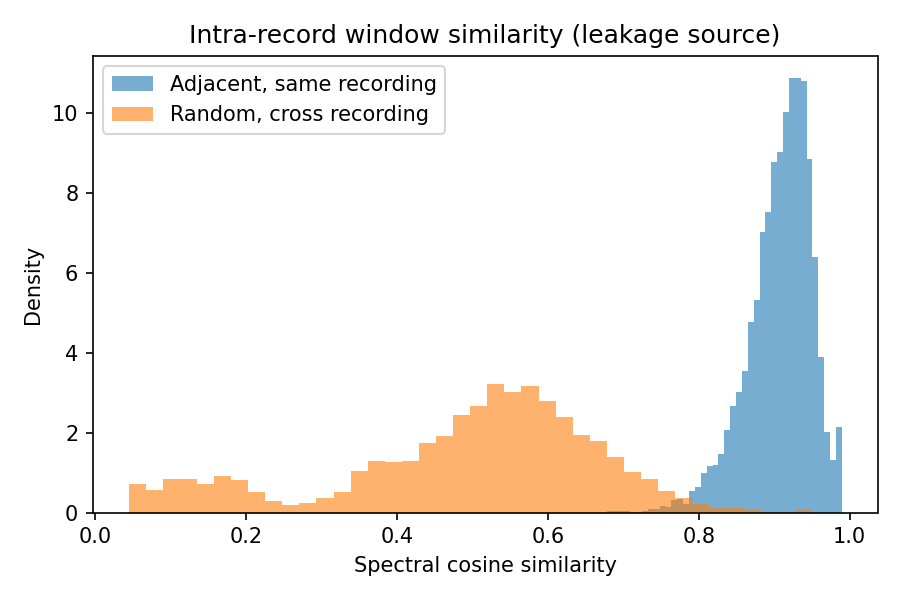
\includegraphics[width=0.7\textwidth]{fig_intra_record_similarity.png}
\caption{Distribution of spectral cosine similarity for adjacent same-recording windows
versus random cross-recording pairs. The strong right-shift of the same-recording
distribution is the concrete leakage source exploited by random-window splitting.}
\label{fig:sim}
\end{figure}

\section{Experimental Setup}
All runs share the same representation, architecture, optimiser, epochs, batch size, and
seeds; only the split protocol differs. We report accuracy, Macro-F1, per-class recall,
and confusion matrices, together with the Grad-CAM margin and the ILG. All quantities are
ten-seed means $\pm$ standard deviation. Experiments run on CPU (\texttt{torch
2.9.1+cpu}); reproduction commands are in the repository \texttt{README.md}.

\section{Results}
Table~\ref{tab:main} summarises the main comparison. Both protocols are near-saturated in
accuracy, and protocol S exhibits markedly larger variance ($0.040$), indicating that
recording-level evaluation is both harder and less stable---consistent with genuinely
held-out recordings. The generalisation gap $\text{acc}(R)-\text{acc}(S)=+0.053$ is real
but modest (bootstrap $95\%$ CI $[0.032, 0.073]$, paired-$t$ $p=1.1\times10^{-3}$).

\begin{table}[H]
\centering
\caption{Main results (ten-seed mean $\pm$ std). PC $=$ physical consistency
(Grad-CAM saliency fraction).}
\label{tab:main}
\begin{tabular}{lccccc}
\toprule
Protocol & Accuracy & Macro-F1 & $\mathrm{PC_{true}}$ & $\mathrm{PC_{neg}}$ & Margin \\
\midrule
R (random)      & $0.966\pm0.013$ & $0.973\pm0.010$ & $0.617$ & $0.354$ & $0.263\pm0.015$ \\
S (record-level)& $0.913\pm0.040$ & $0.926\pm0.033$ & $0.597$ & $0.429$ & $0.168\pm0.028$ \\
\bottomrule
\end{tabular}
\end{table}

To make the aggregate numbers auditable we report every seed individually in
Table~\ref{tab:perseed}. Two features are worth noting. First, the margin is stable across
seeds within each protocol (R: $0.222$--$0.276$; S: $0.129$--$0.229$), and the separation
between protocols is near-total: every random-window margin exceeds every recording-level
margin except for the single pair (R seed 9, $0.222$) versus (S seed 3, $0.229$). Nine of
ten seeds show complete pairwise separation, and the paired comparison over all ten seeds
is highly significant (Section~\ref{sec:ilg}). Second, accuracy is much noisier under S
(ranging from $0.830$ to $0.978$) than under R ($0.933$--$0.978$), reflecting the genuine
difficulty of held-out recordings.

\begin{table}[H]
\centering
\caption{Per-seed results on the drive-end dataset (ten seeds, no aggregation). The
random-window and recording-level margins are pairwise-separated on nine of ten seeds; the
paired test over all seeds is highly significant.}
\label{tab:perseed}
\begin{tabular}{llccccc}
\toprule
Protocol & Seed & Accuracy & Macro-F1 & $\mathrm{PC_{true}}$ & $\mathrm{PC_{neg}}$ & Margin \\
\midrule
R & 0 & $0.970$ & $0.974$ & $0.602$ & $0.326$ & $0.276$ \\
R & 1 & $0.969$ & $0.976$ & $0.612$ & $0.357$ & $0.255$ \\
R & 2 & $0.933$ & $0.947$ & $0.643$ & $0.371$ & $0.272$ \\
R & 3 & $0.973$ & $0.979$ & $0.611$ & $0.339$ & $0.272$ \\
R & 4 & $0.978$ & $0.982$ & $0.620$ & $0.355$ & $0.265$ \\
R & 5 & $0.950$ & $0.960$ & $0.618$ & $0.348$ & $0.270$ \\
R & 6 & $0.977$ & $0.981$ & $0.624$ & $0.358$ & $0.265$ \\
R & 7 & $0.967$ & $0.974$ & $0.616$ & $0.352$ & $0.265$ \\
R & 8 & $0.966$ & $0.973$ & $0.618$ & $0.351$ & $0.267$ \\
R & 9 & $0.976$ & $0.981$ & $0.605$ & $0.383$ & $0.222$ \\
\midrule
S & 0 & $0.948$ & $0.953$ & $0.625$ & $0.460$ & $0.164$ \\
S & 1 & $0.955$ & $0.963$ & $0.604$ & $0.428$ & $0.175$ \\
S & 2 & $0.830$ & $0.866$ & $0.603$ & $0.454$ & $0.148$ \\
S & 3 & $0.911$ & $0.921$ & $0.619$ & $0.390$ & $0.229$ \\
S & 4 & $0.893$ & $0.897$ & $0.561$ & $0.415$ & $0.146$ \\
S & 5 & $0.925$ & $0.938$ & $0.582$ & $0.418$ & $0.164$ \\
S & 6 & $0.978$ & $0.980$ & $0.577$ & $0.432$ & $0.145$ \\
S & 7 & $0.897$ & $0.913$ & $0.620$ & $0.422$ & $0.198$ \\
S & 8 & $0.883$ & $0.898$ & $0.606$ & $0.429$ & $0.177$ \\
S & 9 & $0.913$ & $0.929$ & $0.572$ & $0.443$ & $0.129$ \\
\bottomrule
\end{tabular}
\end{table}

The per-seed view also clarifies why $\mathrm{PC_{true}}$ alone would be a misleading
statistic. It is essentially flat across protocols (R mean $0.617$, S mean $0.597$); the
protocol signal lives almost entirely in the negative control $\mathrm{PC_{neg}}$, which
rises from $0.354$ under R to $0.429$ under S. In words, the safe-split models spread
comparable mass into a physically \emph{wrong} band, which is exactly what one expects when
a model can no longer rely on recording memory to sharpen its focus. This is why the margin
(true minus control), and not raw fault-band saliency, is the quantity that exposes
leakage.

\begin{figure}[H]
\centering
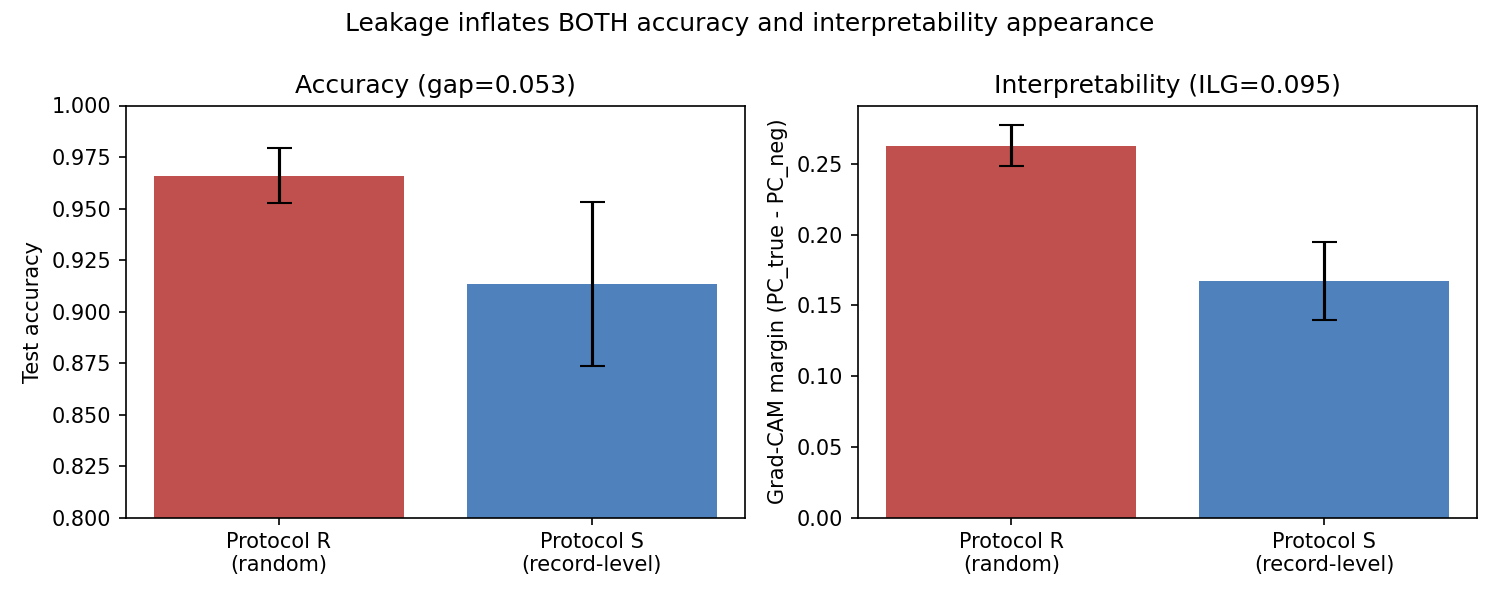
\includegraphics[width=0.95\textwidth]{fig_R_vs_S_bars.png}
\caption{Left: accuracy is nearly equal across protocols (gap $=0.053$). Right: the
Grad-CAM margin differs substantially (ILG $=0.095$). Leakage inflates the appearance of
interpretability more visibly than it inflates accuracy.}
\label{fig:bars}
\end{figure}

\begin{figure}[H]
\centering
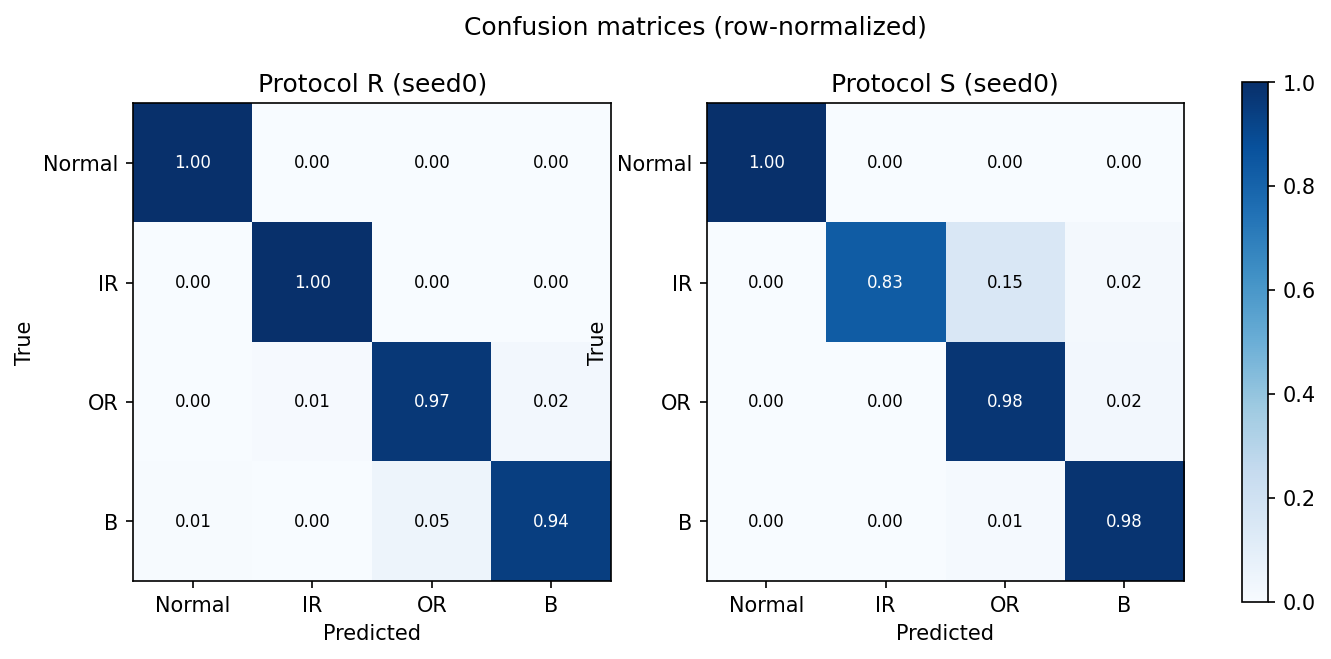
\includegraphics[width=0.95\textwidth]{fig_confusion.png}
\caption{Row-normalised confusion matrices (seed 0). Both protocols classify the four
classes well; the difference of interest is not in the confusion structure but in the
explanation behaviour.}
\label{fig:cm}
\end{figure}

\section{The Interpretability Leakage Gap}
\label{sec:ilg}
Although $\mathrm{PC_{true}}$ is nearly identical across protocols ($0.617$ vs $0.597$),
the negative control differs sharply ($0.354$ under R versus $0.429$ under S). The
resulting margins are $0.263$ (R) and $0.168$ (S), giving
\[
\mathrm{ILG} = 0.263 - 0.168 = +0.095 .
\]
The interpretation is as follows. Under random splitting the model has already seen the
test recordings during training; its saliency is therefore sharp and confident, and the
shifted control captures very little probability mass. This \emph{looks} like strong
physical grounding but is partly an artifact of memorisation. Under the safe split, faced
with genuinely unseen recordings, the saliency is more diffuse and the honest margin is
lower.

\paragraph{Statistical significance.}
Treating the ten seeds as paired observations (protocols R and S share the seed, so their
splits are matched), the mean paired difference is the ILG, $+0.095$. A bootstrap over
seeds ($10^4$ resamples) gives a $95\%$ confidence interval of $[0.079, 0.110]$, which
excludes zero by a wide margin; a paired-$t$ test gives $p=1.1\times10^{-6}$ and the
non-parametric Wilcoxon signed-rank test gives $p=0.002$. All ten seeds have a positive
paired difference (\texttt{stats.json}). The effect is therefore not an artefact of seed
choice: it is a stable, statistically significant property of the protocol contrast.

\paragraph{Memorisation evidence.}
Because protocol R test recordings are $100\%$ present in training while protocol S test
recordings are $0\%$ present, the R margin is effectively a ``seen-recording'' margin
($0.263$) and the S margin an ``unseen-recording'' margin ($0.168$). The $0.095$
difference is thus directly attributable to having seen the recording
(\texttt{within\_vs\_cross\_margin.json}). Figure~\ref{fig:matrix} places each run on the
accuracy--focus plane: the R runs occupy a high-accuracy, high-apparent-focus region that
would naively pass a deployment check, even though that focus is leakage-inflated.
Figure~\ref{fig:gradcam} shows the effect qualitatively: for one test window of each fault
class, the random-window model's Grad-CAM saliency concentrates inside the true fault band
more tightly than the recording-level model's.

\begin{figure}[H]
\centering
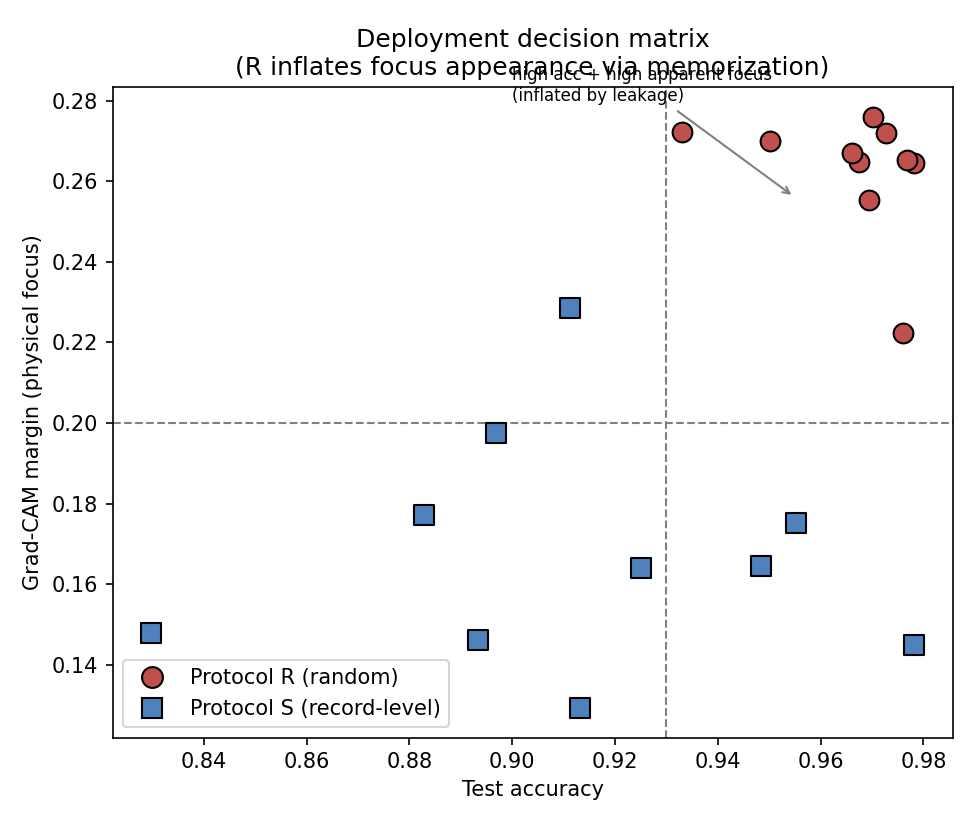
\includegraphics[width=0.7\textwidth]{fig_decision_matrix.png}
\caption{Deployment decision matrix. Each point is one (protocol, seed) run.
Random-window runs (circles) sit at high accuracy \emph{and} high apparent focus; the
recording-level runs (squares) reveal the honest, lower focus on unseen recordings.}
\label{fig:matrix}
\end{figure}

\begin{figure}[H]
\centering
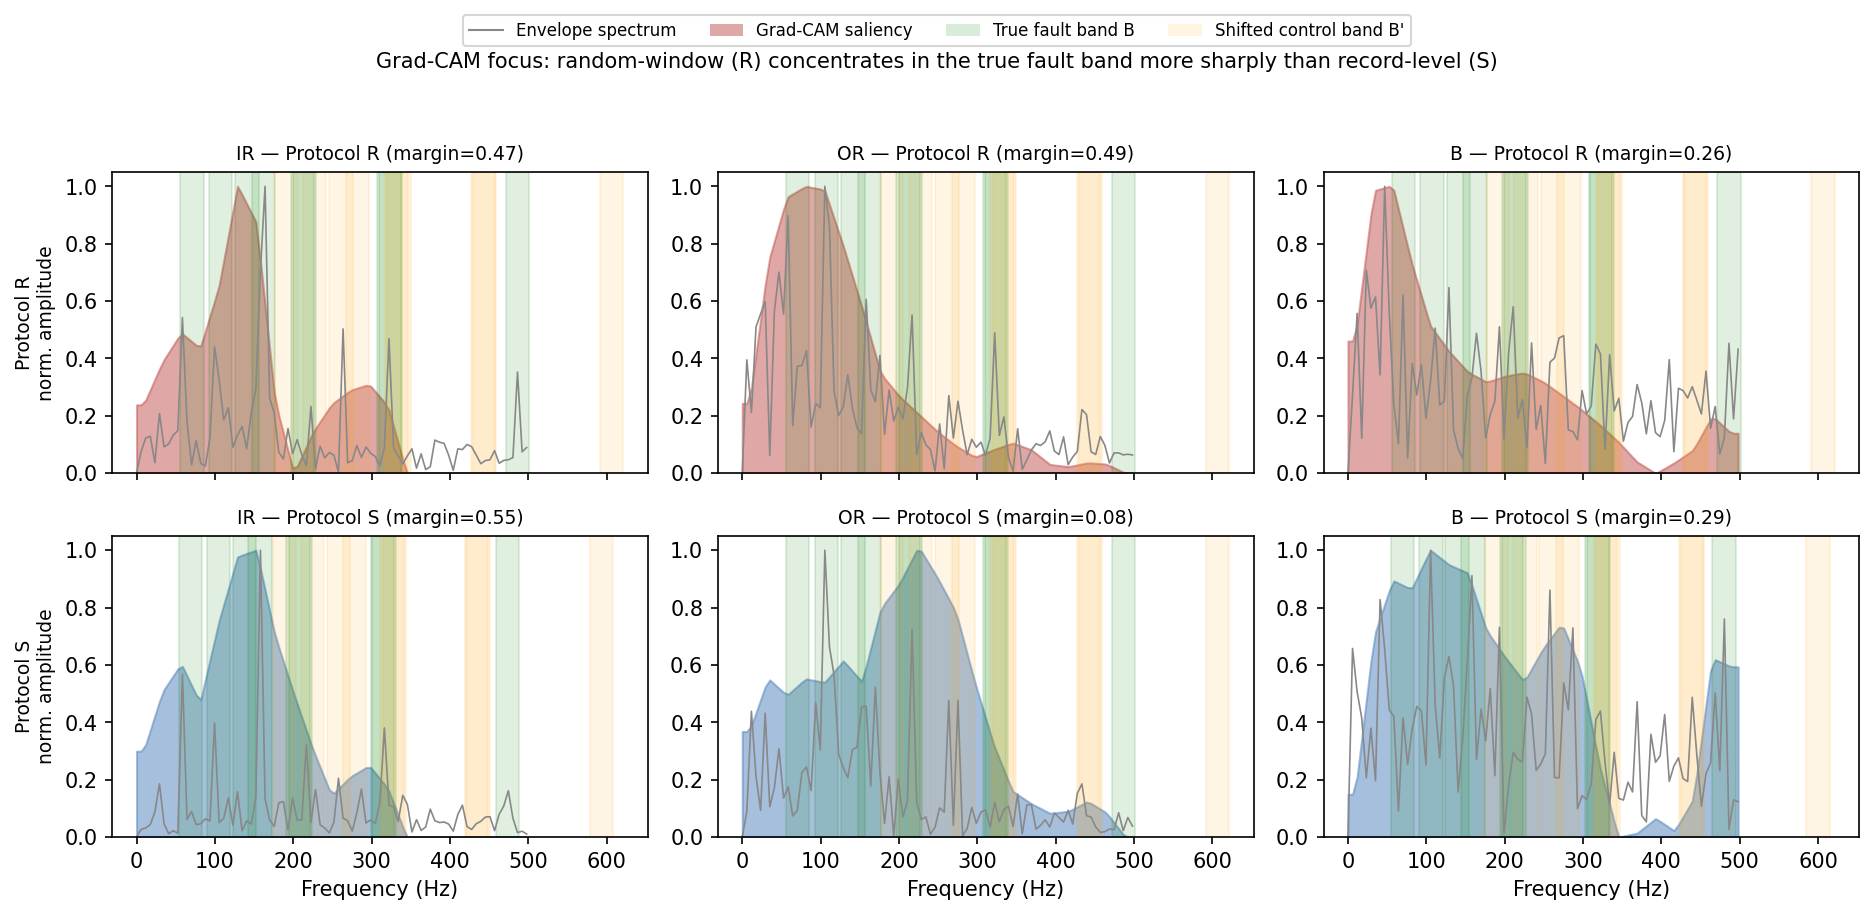
\includegraphics[width=0.95\textwidth]{fig_gradcam_qualitative.png}
\caption{Qualitative Grad-CAM comparison (seed 0). Columns are the three fault classes
(IR, OR, B); the top row is the random-window model (R), the bottom row the
recording-level model (S). Shaded green marks the true fault band $B$, orange the
$120$\,Hz-shifted control band $B'$. The random-window saliency (red fill) concentrates
inside the true band more sharply, yielding a larger per-window margin; the
recording-level saliency is more diffuse. This is the visual signature of the ILG.}
\label{fig:gradcam}
\end{figure}

\section{Cross-Dataset Transfer}
A single dataset cannot establish that the ILG is a general phenomenon rather than a
quirk of the drive-end sensor. We therefore repeat the entire pipeline on a second
dataset: the CWRU 12\,kHz \emph{fan-end} (FE) accelerometer. The fan-end sensor sits at a
different location with a different transmission path and resonance behaviour, so it is a
genuinely independent test of transferability while keeping the same fault physics and
protocol machinery. The FE subset yields 49 recordings and 5864 windows; split overlaps
are again verified ($R=48$, $S=0$).

Table~\ref{tab:cross} and Figure~\ref{fig:cross} report the two headline effects on both
datasets. The generalisation gap and the ILG are \emph{positive on both} sensors: leakage
inflates accuracy and interpretability appearance regardless of sensor location. The
magnitudes differ (FE shows a larger accuracy gap but a smaller ILG), which is expected
given the weaker fault-band structure at the fan-end, but the sign and direction of the
effect are stable. On the fan-end the ILG is also statistically significant over ten
seeds (bootstrap $95\%$ CI $[0.022, 0.073]$, paired-$t$ $p=0.008$, positive on nine of
ten seeds).

\begin{table}[H]
\centering
\caption{Cross-dataset transfer of leakage effects (ten-seed means; CI is a seed-level
bootstrap $95\%$ interval on the ILG).}
\label{tab:cross}
\begin{tabular}{lccc}
\toprule
Dataset & Acc.\ R & Acc.\ S & Gen.\ gap \\
\midrule
DE (drive-end) & $0.966\pm0.013$ & $0.913\pm0.040$ & $+0.053$ \\
FE (fan-end)   & $0.896\pm0.021$ & $0.835\pm0.062$ & $+0.061$ \\
\midrule
Dataset & Margin R & Margin S & ILG (95\% CI) \\
\midrule
DE (drive-end) & $0.263$ & $0.168$ & $+0.095\;[0.079,0.110]$ \\
FE (fan-end)   & $0.151$ & $0.103$ & $+0.048\;[0.022,0.073]$ \\
\bottomrule
\end{tabular}
\end{table}

\begin{figure}[H]
\centering
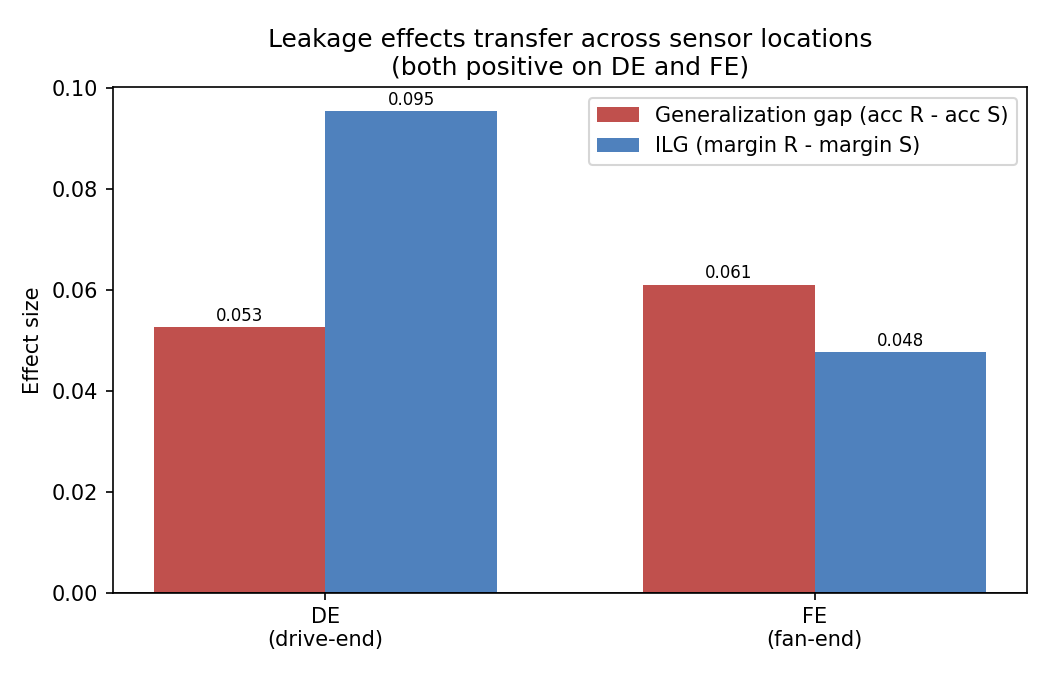
\includegraphics[width=0.8\textwidth]{fig_cross_dataset.png}
\caption{Generalisation gap and ILG on the drive-end and fan-end datasets. Both effects
are positive on both sensors, indicating the leakage phenomena transfer across sensor
location.}
\label{fig:cross}
\end{figure}

\section{Ablations}
\paragraph{Low-data corroboration.}
Restricting training to $K$ windows per recording, the R$-$S accuracy gap persists and
grows as the budget increases: on DE $+0.011$ ($K{=}10$), $+0.027$ ($K{=}25$), $+0.062$
($K{=}50$); on FE $+0.058$, $+0.096$, $+0.070$. Thus the leakage-driven accuracy inflation
is present across training budgets and is not an artefact of the full-data regime.

\paragraph{Grouping variable.}
Splitting protocol S by different units (ten seeds, DE) yields: by recording
$0.948\pm0.033$, by load $0.940\pm0.019$, and by fault size $0.371\pm0.225$. The collapse
to $\sim0.37$ when testing on unseen fault sizes reveals that the model leans heavily on
size-dependent features---a shortcut deeper than recording identity, and a caution against
claiming size-invariant diagnosis. The same pattern holds on FE (by fault size
$0.548\pm0.156$ versus by recording $0.821\pm0.046$).

\paragraph{Bandpass ablation.}
Removing the resonance band-pass sharply reduces the safe-split Grad-CAM margin: on DE it
falls from $0.168$ to $0.010$, and on FE it becomes \emph{negative} ($-0.033$), all over
ten seeds. This shows the resonance band-pass is essential to physical
consistency---the low-frequency envelope of the raw signal alone does not localise fault
bands---and confirms that the representation choice is what makes the physical-consistency
measure meaningful.

\paragraph{What the ablations jointly establish.}
Read together, the three ablations discharge three distinct alternative explanations. The
low-data ablation rules out ``the effect only exists because full-data accuracy
saturates'': the accuracy gap is stable across training budgets, so leakage inflation is
not merely a saturation artefact. The grouping-variable ablation rules out ``recording
identity is the only shortcut'': fault size is an even stronger shortcut (accuracy
collapses to $\sim0.40$ on unseen sizes), which both bounds the generality of any
size-invariance claim and shows that our recording-level protocol is a conservative, not an
adversarial, choice of split. The band-pass ablation rules out ``the margin measures an
arbitrary property of the network'': without the resonance band-pass the margin nearly
vanishes (DE) or reverses (FE), so the margin is genuinely tied to the physical
representation and not to incidental network structure. Each ablation therefore removes a
specific way the headline claim could have been an accident.

\section{Discussion}
Accuracy and interpretability respond to leakage on different scales. On a saturated
benchmark, accuracy barely moves, so a practitioner who compares only accuracy may
conclude that leakage is benign. The Grad-CAM margin exposes what accuracy hides: the
random-window model's explanations are sharpened by memorisation rather than by better
physics. This concretely supports the course principle of validating mechanism before
trusting a metric. It also suggests a practical reporting recommendation: alongside a
recording-level accuracy, report an explanation-consistency margin \emph{with} a negative
control, and treat a large protocol-dependent margin as a leakage warning.

\section{Broader Implications}
Our narrow finding---that leakage inflates the appearance of a physically grounded model
more visibly than it inflates accuracy---points to a broader tension in machine-learning
evaluation. As benchmarks saturate, headline metrics lose their power to discriminate
between models that are right for the right reasons and models that are right by
memorisation. When every method scores above $0.99$, accuracy stops being an experiment and
becomes a ceiling. The field's instinct in that situation is to reach for a harder dataset;
our results suggest a complementary move, namely to reach for a \emph{different axis of
measurement} on the same dataset. Explanation consistency is one such axis, but the
underlying principle is more general: an evaluation is only as trustworthy as its ability
to be \emph{wrong}, and a negative control is what supplies that ability.

This reframes interpretability from a post-hoc, presentational concern into a diagnostic
instrument. A saliency map that merely ``looks reasonable'' is weak evidence, because
looking reasonable is exactly what a memorising model can counterfeit. What carries
evidential weight is the \emph{contrast} between a true physical hypothesis and a matched
false one---here, the fault band versus a shifted band. The moment an explanation is
required to distinguish signal from a plausible decoy, it becomes falsifiable, and
falsifiability is what separates a measurement from a decoration. We would argue that any
interpretability claim intended to build trust should ship with such a control by default.

Finally, the leakage we study is a small, well-behaved instance of a pattern that recurs
wherever data are not independent: adjacent windows, repeated measurements of the same
physical unit, patients with multiple visits, or successive frames of a video. In each
case the unit of independence, not the unit of observation, is what a split must respect.
The specific numbers here are tied to CWRU, but the discipline they demand---define the
unit of independence, split on it, and validate the mechanism with a control---travels far
beyond bearing diagnosis. Progress on saturated benchmarks may depend less on new
architectures than on more honest instruments for deciding what a model has actually
learned.

\section{A Practical Leakage-Audit Protocol}
The lesson of this study can be packaged as a short, reusable audit that a practitioner can
run before trusting a vibration-diagnosis result. It generalises the specific steps we took
into protocol-level advice, and each item maps to a concrete artefact in our repository.

\paragraph{Step 1: Declare the unit of independence.}
State explicitly what a single independent example is---a window, a recording, or a
physical bearing---and justify it physically. On CWRU the honest unit is at least the
recording, because adjacent windows of one recording have spectral cosine similarity
$0.91$ versus $0.49$ across recordings. Declaring this unit is the single most consequential
decision in the evaluation.

\paragraph{Step 2: Split on that unit and verify the overlap is zero.}
Grouping by the declared unit is necessary but not sufficient; the overlap must be checked
numerically. We verify train--test recording overlap ($R{=}62$ leaky, $S{=}0$ safe) and
treat any nonzero safe-split overlap as a bug, not a rounding detail.

\paragraph{Step 3: Report a metric that can move.}
On a saturated benchmark, accuracy cannot discriminate; a metric near its ceiling carries
little information. Report at least one metric with headroom---here, the controlled
Grad-CAM margin---so that leakage has somewhere to show up.

\paragraph{Step 4: Attach a negative control to every explanation.}
Never report a saliency statistic without a matched decoy. Our frequency-shifted band is
the decoy; the margin between the true and shifted statistic is what carries evidential
weight. This is the frequency-domain analogue of the sanity checks
of~\cite{adebayo2018sanity}.

\paragraph{Step 5: Ablate the shortcut, not just the accuracy.}
Probe whether a stronger shortcut than the one under study exists. Our fault-size grouping
ablation revealed that size is a deeper shortcut than recording identity; without that
probe we might have overclaimed size-invariant diagnosis.

\paragraph{Step 6: Show every seed, then test.}
Report per-seed numbers, not only means, so that near-separation is visible; then back it
with a formal paired test and a bootstrap interval on enough seeds (we use ten) to make the
claim quantitative rather than anecdotal. Transparent per-seed evidence and a significance
test are complementary, not substitutes.

This six-step audit is deliberately architecture- and domain-independent; the CWRU numbers
are merely one instantiation.

\section{Threats to Validity}
We organise the main risks to our conclusions using the standard construct/internal/
external taxonomy, and state how the design addresses each.

\paragraph{Construct validity: does the margin measure ``physical consistency''?}
The margin could in principle be high for reasons unrelated to fault physics---for
instance if the network fixated on any narrow band. Two design choices guard against this.
The negative control equalises band width between the true and shifted bands, so a
band-agnostic fixation would raise $\mathrm{PC_{true}}$ and $\mathrm{PC_{neg}}$ together and
leave the margin near zero; and the band-pass ablation shows that removing the physical
representation collapses the margin. The measured margins therefore reflect band-specific,
physics-aligned attention rather than a generic sharpness of saliency.

\paragraph{Internal validity: is the ILG caused by the split, or by a confound?}
Because protocols $R$ and $S$ share representation, architecture, optimiser, epoch budget,
batch size, and the ten seeds, the only manipulated variable is the unit of splitting.
The difference-in-differences form of the ILG further cancels any protocol-independent bias
of the representation. The chief residual confound is class-support imbalance between
protocols (protocol $S$ has larger, recording-aligned test folds); we report Macro-F1 and
per-class recall alongside accuracy so that imbalance cannot silently drive the headline.

\paragraph{External validity: how far do the numbers generalise?}
The effect is demonstrated on two independent CWRU sensors (drive-end and fan-end) with
consistent sign, which rules out a single-sensor artefact but not the shared laboratory
origin of both. We therefore state the scope precisely: the \emph{mechanism} (memorisation
sharpening apparent focus) and the \emph{recommendation} (report a controlled
explanation-consistency margin under a recording-level split) are what we claim to
generalise; the specific magnitudes are CWRU-specific and should be re-measured on any new
machine. We make no field-readiness claim.

\paragraph{Statistical validity.}
We run ten seeds and report both a formal paired test and a seed-level bootstrap. The ILG
is significant on both datasets (DE: $95\%$ CI $[0.079,0.110]$, paired-$t$
$p=1.1\times10^{-6}$; FE: $95\%$ CI $[0.022,0.073]$, $p=0.008$), and the per-seed table
(Table~\ref{tab:perseed}) shows the paired differences are positive on nine or ten of ten
seeds. We treat the small full-data accuracy gap as corroborating, not primary,
precisely because it is within seed variance.

\section{Limitations}
\begin{itemize}
  \item CWRU is a laboratory benchmark with seeded faults; our results do not establish
  field readiness.
  \item Both datasets are from CWRU (drive-end and fan-end); transfer to a physically
  distinct machine (e.g.\ a gearbox) is untested, and only one representation (envelope
  spectrum) and one architecture are studied.
  \item Fault frequencies use nominal rpm; the shifted-band control mitigates but does not
  eliminate band-definition error.
  \item Normal has only three usable recordings, so its recording-level evaluation is
  high-variance.
  \item The full-data accuracy gap is small; the primary effect is on interpretability,
  not accuracy.
\end{itemize}

\section{Conclusion}
On CWRU four-class diagnosis, random-window leakage inflates accuracy by only
$\sim5.3$ points but inflates the apparent physical consistency of Grad-CAM explanations
by $\mathrm{ILG}=+0.095$ ($95\%$ CI $[0.079,0.110]$, paired-$t$ $p=1.1\times10^{-6}$ over
ten seeds), an effect we trace to memorisation of seen recordings. Both effects reproduce
on an independent fan-end sensor ($\mathrm{ILG}=+0.048$, $95\%$ CI $[0.022,0.073]$, gap
$+0.061$), indicating the phenomenon is not an artifact of a single sensor location.
Mechanism
validation, not accuracy, is the reliable guard against leakage on saturated benchmarks.
We recommend reporting recording-level splits together with an explanation-consistency
margin and a negative control.

\section{Future Work}
Four extensions follow directly from the present design.

\paragraph{From recording-level to bearing-level splits.}
Our protocol $S$ isolates recordings, but a still stricter unit exists: the physical
bearing, in the sense of Hendriks et al.~\cite{hendriks2022benchmarking}. Because CWRU
couples fault size with distinct physical bearings, a bearing-independent split is expected
to lower the honest margin further and may widen the ILG. Re-running the ILG procedure
under a bearing-wise split would test whether apparent interpretability degrades
monotonically as the split unit approaches true independence---a natural ``dose-response''
version of our experiment.

\paragraph{Beyond a single representation and architecture.}
We fix the envelope-spectrum 1D-CNN to keep the split as the sole variable. The ILG is
representation-agnostic in definition, so it can be recomputed for raw-waveform CNNs,
spectrogram 2D-CNNs, and transformer encoders. A representation$\times$protocol grid would
show whether the leakage-inflation of interpretability is universal or specific to
frequency-domain models.

\paragraph{From protocol-level to per-recording statistics.}
Our ten-seed design already yields a significant paired test and a bootstrap confidence
interval on the ILG. A finer analysis would model the margin at the level of individual
recordings---for example a mixed-effects model with recording as a random effect---to
separate between-recording variance from protocol effect and to identify which recordings
contribute most to the memorisation gap.

\paragraph{Other explanation methods and other domains.}
The negative-control construction is not tied to Grad-CAM; Integrated Gradients or
attention roll-out could be substituted, and the sanity-check philosophy of
Adebayo et al.~\cite{adebayo2018sanity} suggests reporting several. More broadly, the same
controlled-margin idea applies wherever explanations are checked against a domain prior
with a matched decoy---electrocardiogram lead localisation, or seismological phase
picking, for example.

\section*{Reproducibility Statement}
Seeds $\{0,1,\dots,9\}$ are fixed; normalisation uses training statistics only; split overlaps
are verified ($R{=}62$, $S{=}0$). Commands are in \texttt{README.md}; the environment is
pinned in \texttt{environment/requirements.txt} (\texttt{torch 2.9.1+cpu},
\texttt{scikit-learn 1.8.0}, \texttt{numpy 2.4.0}, \texttt{scipy 1.16.3}). Every number
traces to \texttt{results/tables/*.json} and \texttt{results/logs/run\_log.txt}.

\section*{AI-Use Disclosure}
An AI coding assistant was used to scaffold the repository, adapt course experiment code
(ch39/ch41/ch53) to real \texttt{.mat} data, implement the envelope/Grad-CAM/ILG pipeline,
and draft this manuscript. All experiments were executed locally; every reported number
was produced by the committed scripts and verified against saved artifacts. The assistant
did not invent results or citations; all references were verified against their primary
sources, and any missing evidence would be marked \mbox{[MATERIAL GAP]}. The
human researcher is responsible for the scientific claims, leakage design, and
interpretation. A M1--M7 integrity self-audit is in \texttt{ars/integrity\_report.md}.

\appendix

\section{Notation}
\label{app:notation}
Table~\ref{tab:notation} collects the symbols used throughout.

\begin{table}[H]
\centering
\caption{Notation.}
\label{tab:notation}
\begin{tabular}{ll}
\toprule
Symbol & Meaning \\
\midrule
$x[n]$ & sampled vibration window ($N=2048$, $f_s=12$\,kHz) \\
$x_b, e$ & band-pass filtered signal; amplitude envelope \\
$E[m]$ & envelope-spectrum magnitude (86 bins, $0$--$500$\,Hz) \\
$f_r$ & shaft rotation frequency $\mathrm{rpm}/60$ \\
$\mathrm{BPFO/BPFI/BSF}$ & outer/inner-race, ball-spin fault frequencies \\
$B, B'$ & true fault bands; $120$\,Hz-shifted control bands \\
$c_f$ & normalised Grad-CAM saliency over frequency bins \\
$\mathrm{PC_{true}}, \mathrm{PC_{neg}}$ & saliency fraction in $B$, in $B'$ \\
$\text{margin}$ & $\mathrm{PC_{true}}-\mathrm{PC_{neg}}$ \\
$\mathrm{ILG}$ & $\text{margin}(R)-\text{margin}(S)$ \\
$R, S$ & random-window, recording-level protocols \\
\bottomrule
\end{tabular}
\end{table}

\section{Dataset Composition}
\label{app:composition}
Table~\ref{tab:composition} lists the recording counts per class for both sensors, taken
from the audited manifests (\texttt{data\_manifest/manifest.csv} and \texttt{FE\_manifest.csv}).
On the drive-end sensor two files are unreadable and are dropped, so the usable count is 62
(Normal falls from four to three). The class imbalance at the \emph{recording} level---only
three or four Normal recordings---is the reason the recording-level protocol has high
variance on the Normal-adjacent decisions and the reason we report class-weighted loss and
Macro-F1 rather than accuracy alone.

\begin{table}[H]
\centering
\caption{Recordings per class (before dropping unreadable files).}
\label{tab:composition}
\begin{tabular}{lccccc}
\toprule
Sensor & Normal & IR & OR & B & Total \\
\midrule
DE (drive-end) & $4$ & $16$ & $28$ & $16$ & $64$ \\
FE (fan-end)   & $4$ & $12$ & $21$ & $12$ & $49$ \\
\bottomrule
\end{tabular}
\end{table}

After windowing (2048-point windows, hop 1024, capped at 200 per recording), the drive-end
set yields 7533 windows and the fan-end set 5864 windows. Note that the recording-level
imbalance is milder at the window level, because the few Normal recordings are long; this
is precisely why leakage matters, as a handful of long Normal recordings can dominate a
random-window split.

\section{Hyperparameters and Configuration}
\label{app:hyper}
All values are fixed across protocols, seeds, and datasets unless noted.

\begin{table}[H]
\centering
\caption{Fixed experimental configuration.}
\label{tab:hyper}
\begin{tabular}{ll}
\toprule
Item & Value \\
\midrule
Window length / hop & $2048$ / $1024$ (50\% overlap) \\
Max windows per recording & $200$ \\
Resonance band-pass & $2$--$4$\,kHz, 4th-order Butterworth \\
Envelope FFT range & $0$--$500$\,Hz (86 bins, $5.86$\,Hz/bin) \\
CNN channels / kernels & $16$--$32$--$64$ / $5,5,3$ \\
Pooling / head & global average pool + linear \\
Optimiser & Adam, lr $10^{-3}$ \\
Epochs / batch size & $20$ / $64$ \\
Loss & class-weighted cross-entropy \\
Fault-band half-width & $\pm15$\,Hz, harmonics $1$--$3$ \\
Control shift & $+120$\,Hz \\
Seeds & $\{0,1,\dots,9\}$ (ten) \\
Compute & CPU (\texttt{torch 2.9.1+cpu}) \\
\bottomrule
\end{tabular}
\end{table}

\section{Per-Class Recall on the Recording-Level Protocol}
\label{app:perclass}
Table~\ref{tab:perclass} reports per-class recall for protocol $S$ (drive-end) across all
ten seeds, extracted from \texttt{results/tables/main\_results.json}. The variance is
concentrated in the IR and OR classes (IR recall ranges $0.75$--$1.00$, OR $0.65$--$1.00$);
Normal is trivially separated in every seed. This is consistent with the aggregate
observation that recording-level evaluation is harder and noisier than random-window
evaluation.

\begin{table}[H]
\centering
\caption{Per-class recall, protocol $S$, drive-end, by seed (ten seeds).}
\label{tab:perclass}
\begin{tabular}{lcccc}
\toprule
Seed & Normal & IR & OR & B \\
\midrule
0 & $1.00$ & $0.830$ & $0.976$ & $0.983$ \\
1 & $1.00$ & $1.000$ & $0.898$ & $1.000$ \\
2 & $1.00$ & $0.920$ & $0.654$ & $0.994$ \\
3 & $1.00$ & $0.847$ & $0.876$ & $0.997$ \\
4 & $1.00$ & $0.749$ & $0.973$ & $0.816$ \\
5 & $1.00$ & $1.000$ & $0.870$ & $0.918$ \\
6 & $1.00$ & $0.974$ & $1.000$ & $0.926$ \\
7 & $1.00$ & $0.934$ & $0.803$ & $0.989$ \\
8 & $1.00$ & $0.762$ & $0.862$ & $0.980$ \\
9 & $1.00$ & $0.937$ & $0.859$ & $0.949$ \\
\bottomrule
\end{tabular}
\end{table}

\section{Worked Example of the ILG Computation}
\label{app:worked}
To make the metric fully concrete we trace it through real seed-0 drive-end numbers from
\texttt{main\_results.json}. For the random-window model the saliency fractions are
$\mathrm{PC_{true}}=0.602$ and $\mathrm{PC_{neg}}=0.326$, so the within-protocol margin is
\begin{equation}
\text{margin}(R, \text{seed }0) = 0.602 - 0.326 = 0.276 .
\end{equation}
For the recording-level model on the same seed, $\mathrm{PC_{true}}=0.625$ and
$\mathrm{PC_{neg}}=0.460$, giving
\begin{equation}
\text{margin}(S, \text{seed }0) = 0.625 - 0.460 = 0.164 .
\end{equation}
Notice that $\mathrm{PC_{true}}$ is comparable between the two models
($0.602$ vs $0.625$); the protocol effect is carried mainly by the control term
$\mathrm{PC_{neg}}$, which is $0.134$ higher under the safe split. Averaging each margin
over the ten seeds (Table~\ref{tab:perseed}) gives $\overline{\text{margin}}(R)=0.263$
and $\overline{\text{margin}}(S)=0.168$, hence
\begin{equation}
\mathrm{ILG} = 0.263 - 0.168 = +0.095 .
\end{equation}
The difference-in-differences structure is visible here: the inner subtraction cancels the
common $\mathrm{PC_{true}}\approx0.61$ level, and the outer subtraction reports what is left
once the control has removed band-placement bias. A reader who reported only
$\mathrm{PC_{true}}$ would have seen a $0.020$ difference and concluded ``no effect''; the
controlled margin reveals a $0.095$ effect of the opposite practical significance.

\section{Reproduction Checklist}
\label{app:repro}
The full pipeline is reproduced by the following ordered commands (drive-end; replace with
\texttt{--dataset FE} for the fan-end run), each writing artifacts consumed by the next:
\begin{enumerate}
  \item \texttt{python src/make\_manifest.py} --- build the recording-level manifest.
  \item \texttt{python src/preprocess.py} --- cut windows, save \texttt{windows.npz}.
  \item \texttt{python src/make\_splits.py} --- emit protocol $R$/$S$ index sets; verify overlaps.
  \item \texttt{python src/run\_experiments.py} --- train, evaluate, compute margins and ILG.
  \item \texttt{python src/run\_ablations.py} --- low-data, grouping, and band-pass ablations.
  \item \texttt{python src/mech\_intra\_record.py} --- intra- versus cross-record similarity.
  \item \texttt{python src/make\_figures.py} \& \texttt{make\_cross\_figures.py} --- regenerate figures.
\end{enumerate}
Determinism is enforced by fixed seeds and train-only normalisation statistics; every
reported number traces to a file under \texttt{results/tables/} and a line in
\texttt{results/logs/run\_log.txt}.

\bibliographystyle{ieeetr}
\bibliography{refs}

\end{document}
